\chapter{Concentration Pre-Process Fan-out (CPPF)}

CPPF stands for Concentration PRe-Process Fan-out. This is part of CMS L1 trigger. This was installed during the L1 trigger Phase I upgrade of the CMS. This processes data from End-cap Resistive Plate Chamber (RPC) and overlap region of Barrel RPC detector, in a stage before Endcap Muon Track Finder (EMTF) and Overlap Muon Track Finder (OMTF) stage.

The hardware components of CPPF system, include eight CPPF cards, two MicroTCA Carrier Hub (MCH) cards including a commercial MCH module and a CERN custom designed AMC13 module, an all these cards are mounted in one $\mu$TCA shift.

For the offline software, both CPPF Unpacker and Emulator are developed. The unpacker is responsible for unpacking CPPF data which are sent to DAQ system. On the other hand, the emulator simulates the algorithm function of CPPF firmware. In all, the unpacker and emulator are used to do physical analysis for recorded CPPF DAQ data, then we can evaluate the CPPF system function in global running based on the analysis result.

\section{CPPF Unpacker}
CPPF Unpacker software (Unpacker) is used to unpack the CPPF records in the Data Acquisition (DAQ) system.
% , from Raw data. This converts the Raw data into software-oriented digital data and packaged into new cases for subsequent objects
CPPF unpacker is based on the CMS Software (CMSSW). Its working involves following tasks:
\begin{itemize}
    \item The unpacker read the raw data recorded by the CPPF system in the DAQ system and transfer the data into software-oriented digital data for subsequent analysis
    \item The CPPF hardware uploads two types of data to the DAQ system, namely RPC data received by CPPF (Input data) and data (output data) to be sent to EMTF after CPPF pre-processing. So, the de-packetizer also includes two parts, namely the input data de-packetizer and the output data de-packetizer.
    \item At last unpacker packs the transformed data into new cases in a certain format, having necessary information for the physical analysis requirements. Also, the output format should be similar to the emulator.
\end{itemize}

\section{CPPF Emulator}
Each sub-system of the CMS experiment L1 trigger system has a corresponding simulator to verify and check its hardware function. The input data of the emulator can be obtained from Monte-Carlo simulation or from real data which is the input part of the data using which it is unpacked from CPPF. The output data of the emulator is used to compare with the CPPF unpacker. 

To ensure the data quality, in real time, the comparison information was implemented to the online Data Quality Monitor (DQM). The workfow is shown in Fig.~\ref{fig:CPPF_unpacker_emulator_workflow}.
If everything is working fine then unpacker and emulator should match. We compared the unpacker and emulator as shown in Fig.~\ref{fig:CPPF_unpacker_emulator_comparison_1},~\ref{fig:CPPF_unpacker_emulator_comparison_2} and ~\ref{fig:CPPF_unpacker_emulator_comparison_3}. It was noted that the discripency between the unpacker and emulator is $<$ 1\% level.

\begin{figure*}[htb]
  \centering
%   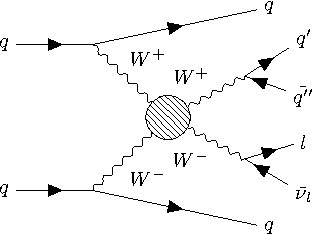
\includegraphics[width=0.33\textwidth]{Images/VBS_Studies/Figure_001-a.pdf}
  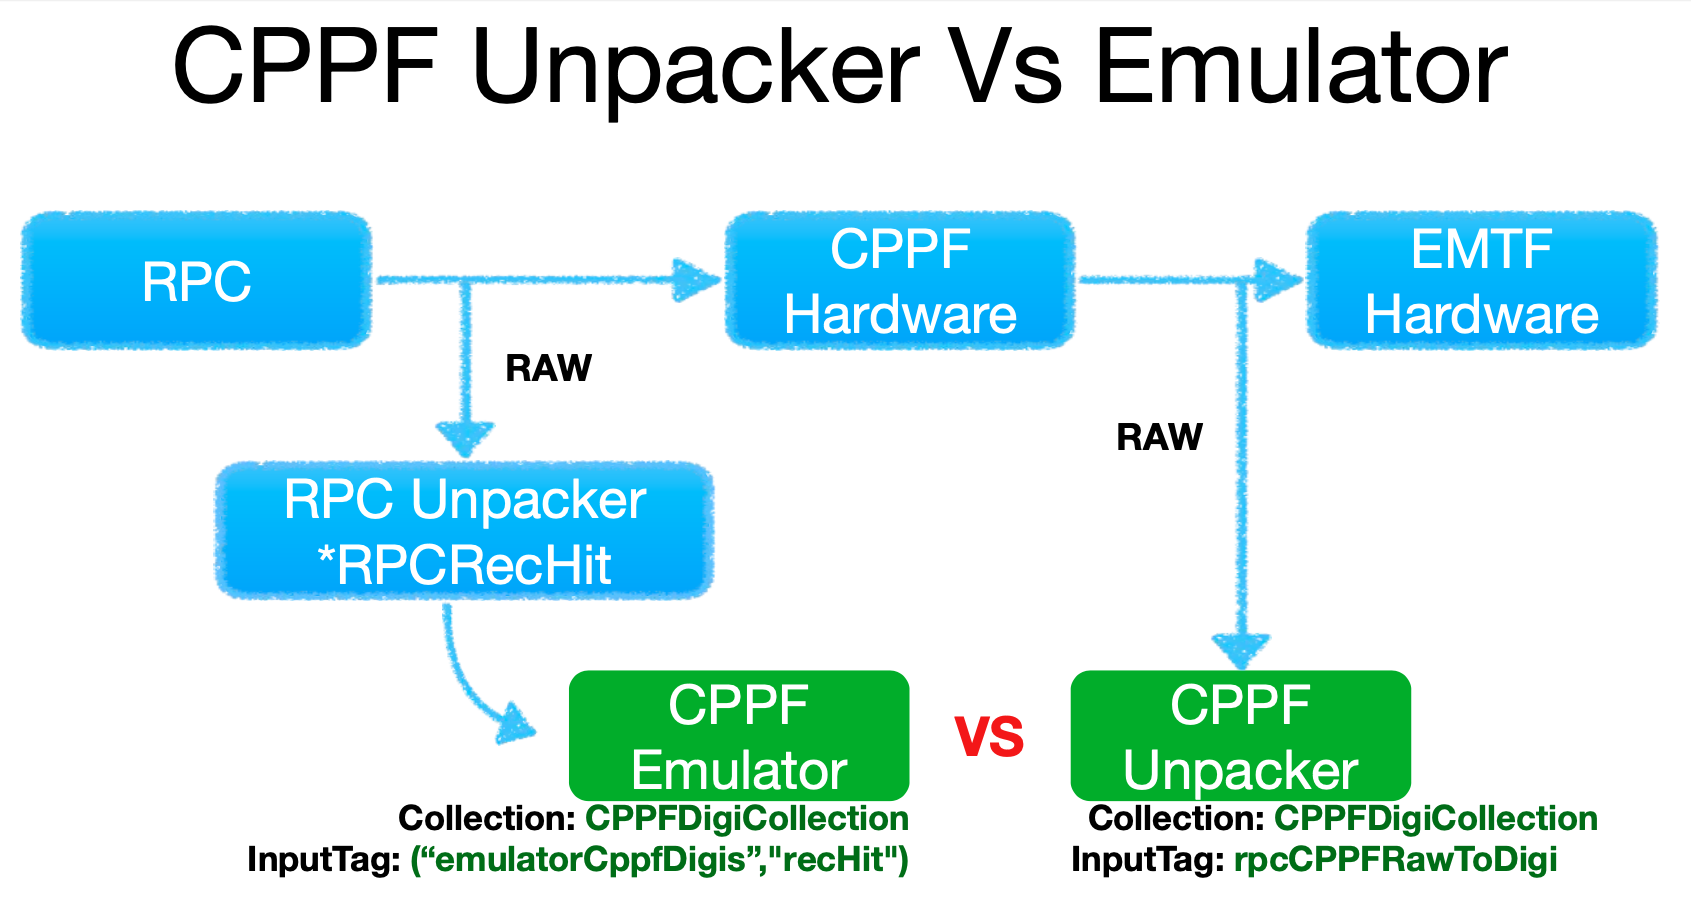
\includegraphics[width=0.95\textwidth]{Images/CPPF/CPPF_unpacker_emulator_workflow.png}
\caption{CPPF unpacker and emulator workflow} \label{fig:CPPF_unpacker_emulator_workflow}
\end{figure*}


\begin{figure*}[htb]
  \centering
  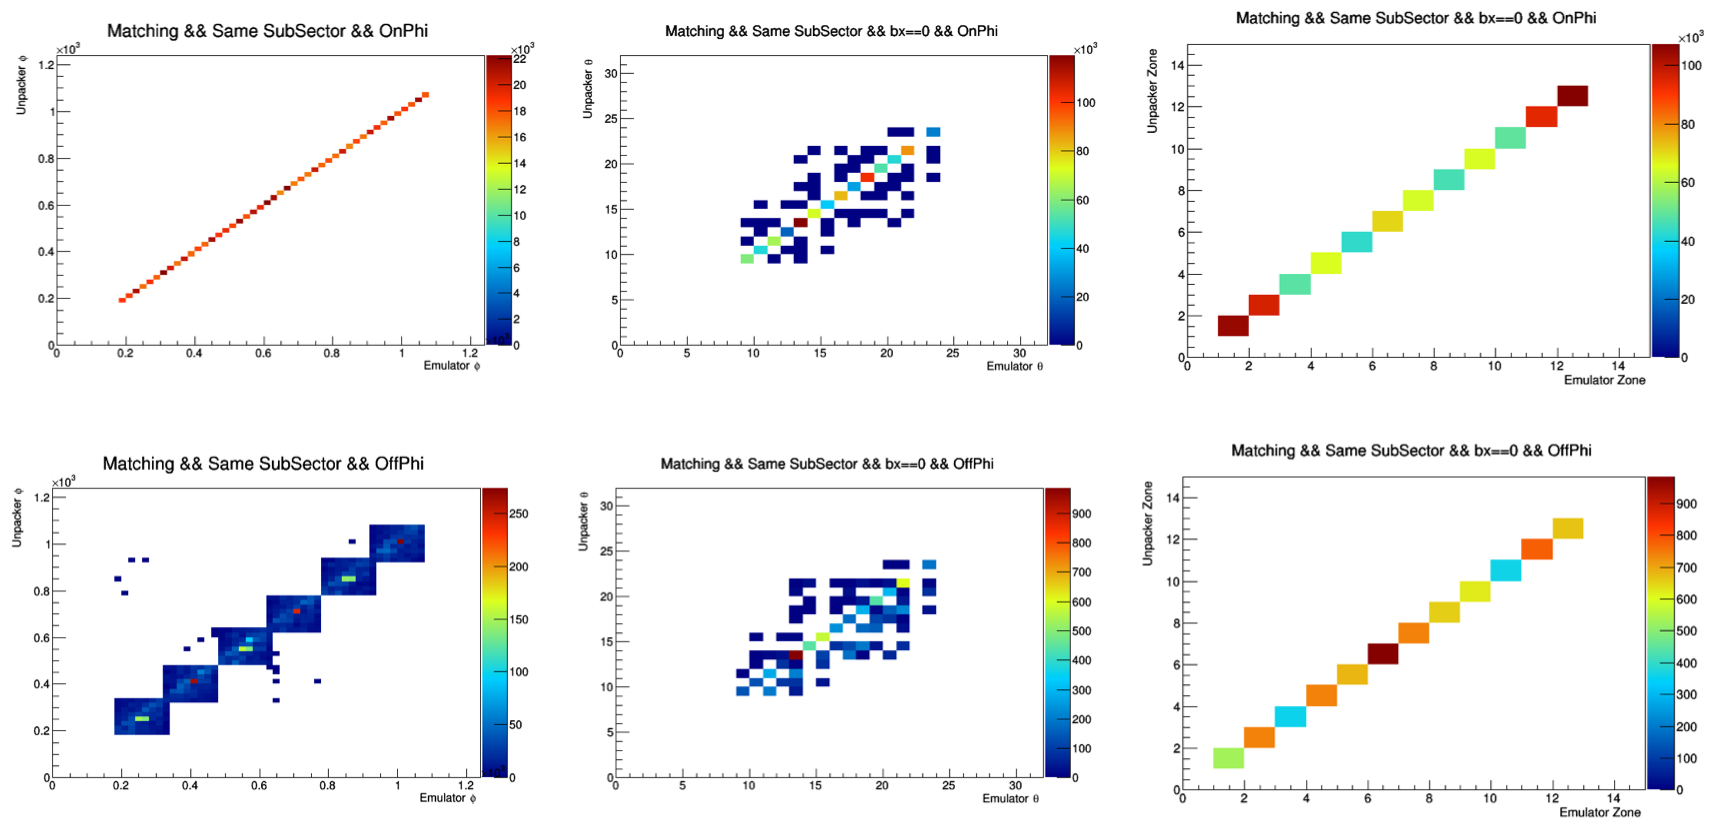
\includegraphics[width=0.95\textwidth]{Images/CPPF/CPPF_UnpEmu_Comparison_01.png}
\caption{2D comparison of CPPF unpacker and emulator} \label{fig:CPPF_unpacker_emulator_comparison_1}
\end{figure*}

\begin{figure*}[htb]
  \centering
  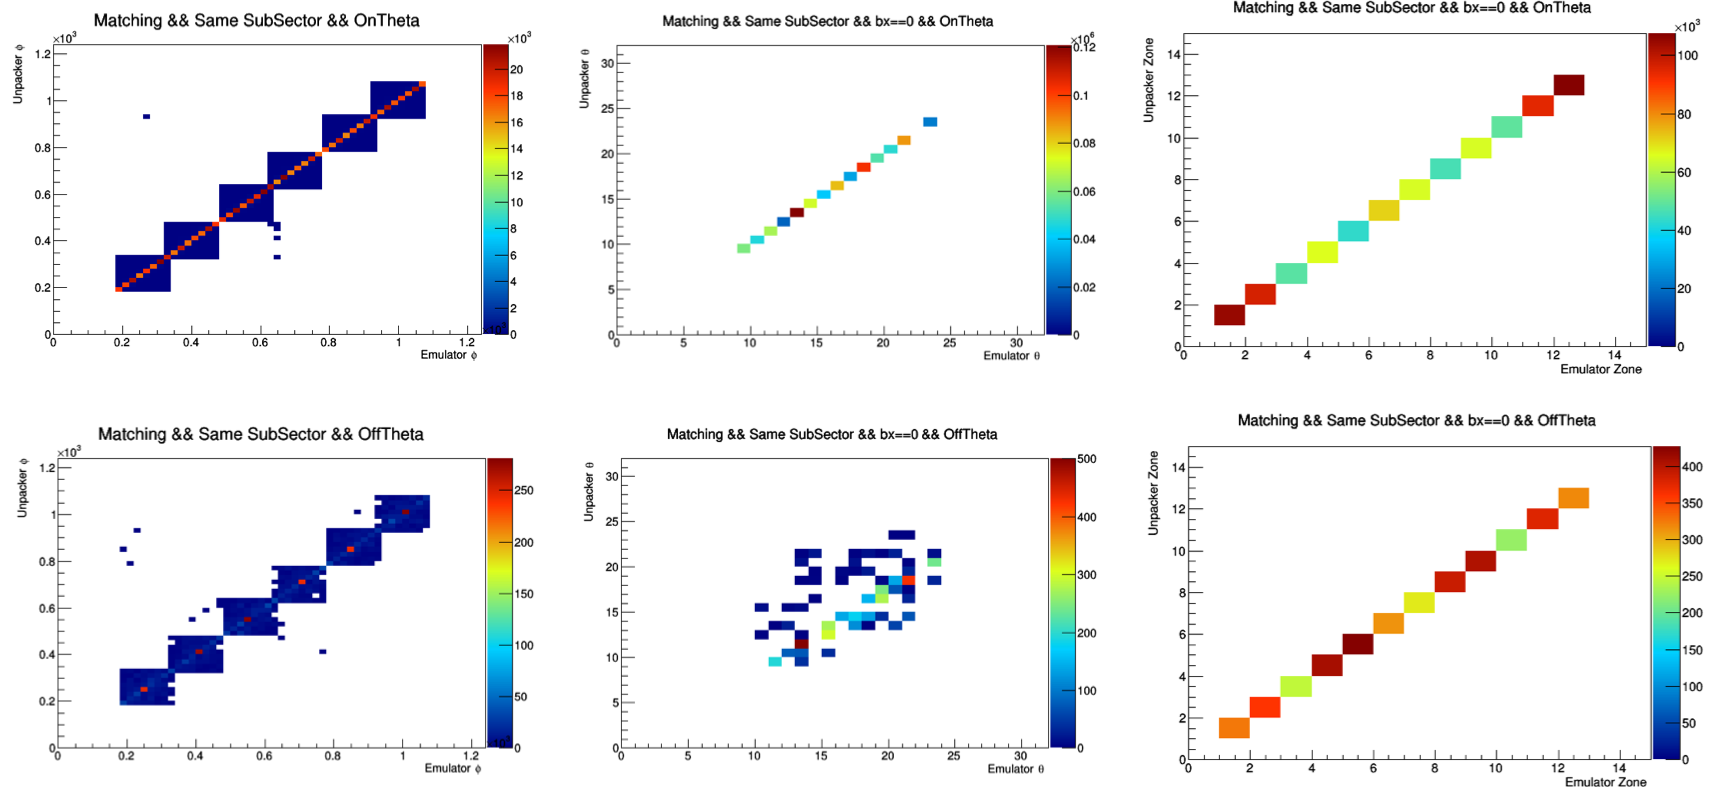
\includegraphics[width=0.95\textwidth]{Images/CPPF/CPPF_UnpEmu_Comparison_13.png}
\caption{2D comparison of CPPF unpacker and emulator} \label{fig:CPPF_unpacker_emulator_comparison_2}
\end{figure*}

\begin{figure*}[htb]
  \centering
  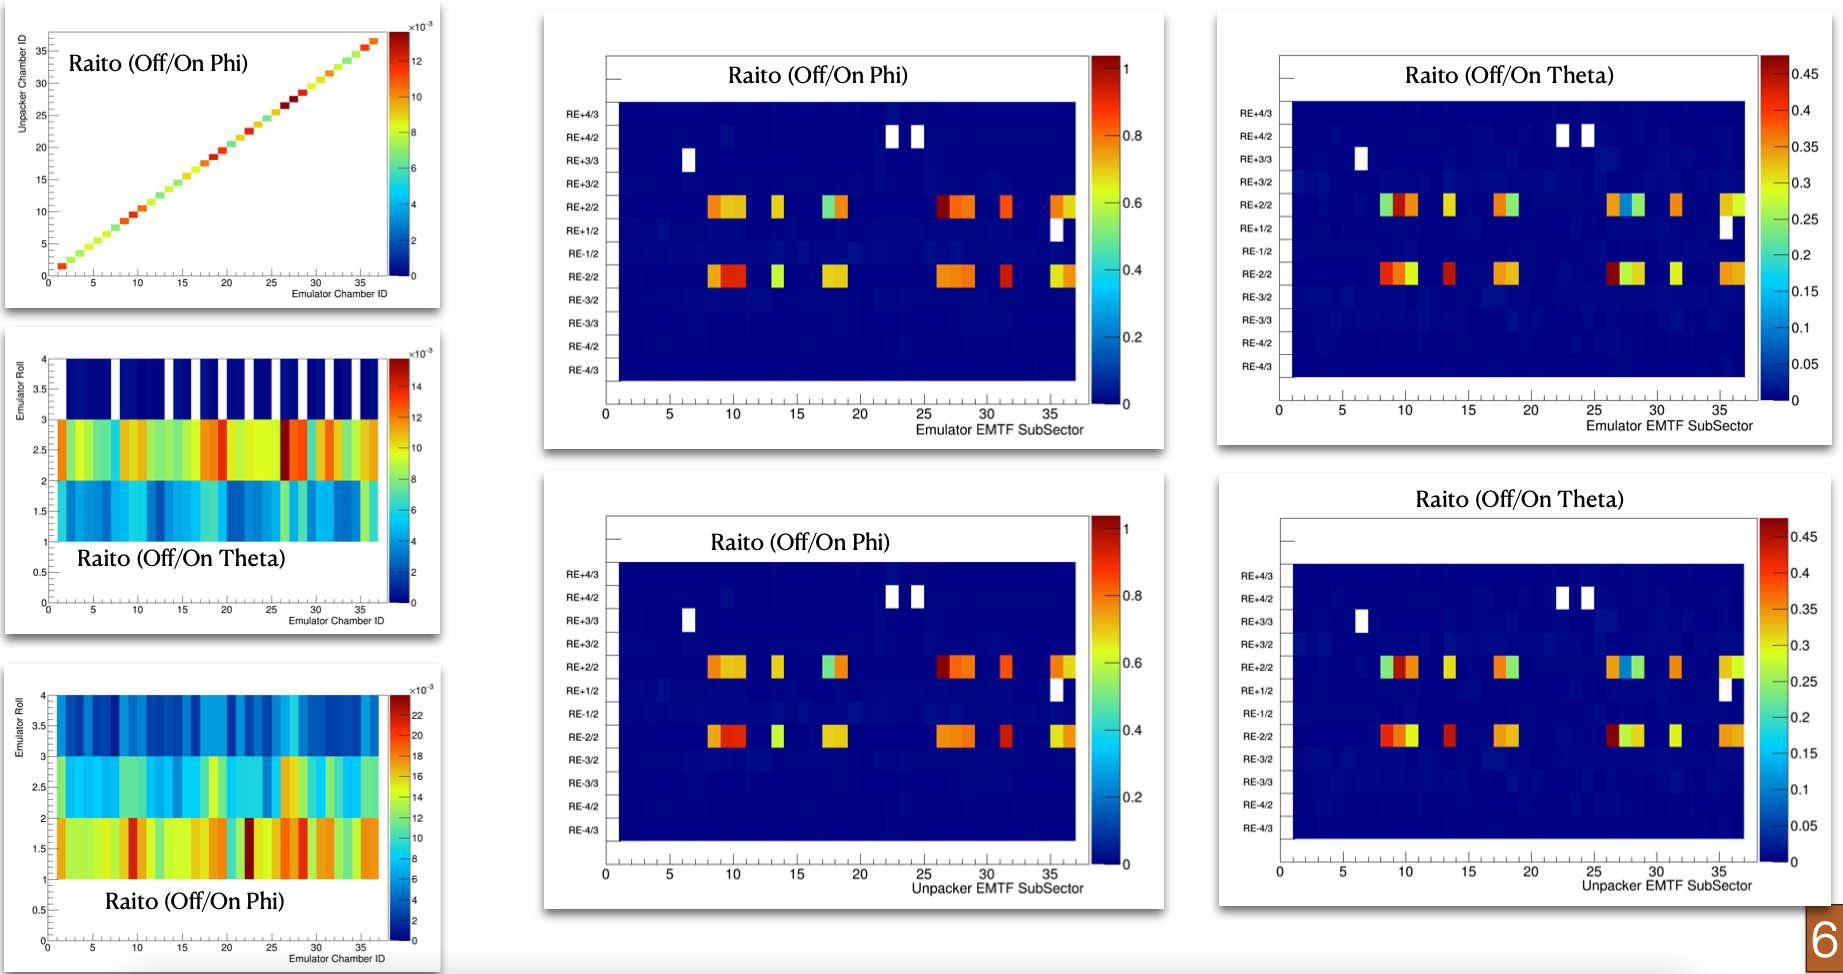
\includegraphics[width=0.95\textwidth]{Images/CPPF/CPPF_UnpEmu_Comparison_28.png}
\caption{2D comparison of CPPF unpacker and emulator} \label{fig:CPPF_unpacker_emulator_comparison_3}
\end{figure*}